\documentclass[10pt,twocolumn]{article}

\usepackage[a4paper,margin=0.75in]{geometry}
\usepackage{booktabs}
\usepackage{tabularx}
\usepackage{graphicx}
\usepackage{subcaption}
\usepackage{enumitem}
\usepackage{xcolor}
\usepackage[hidelinks]{hyperref}
\usepackage{times}

\newcommand{\dataset}{Nemotron-Personas-France}
\newcommand{\ifop}{IFOP}
\newcommand{\stance}{\textit{stance}}
\newcommand{\score}{\textit{support\_score}}

\title{Simulating Public Opinion with Large Language Models:\\A Persona-Based Study of French Pension Reform Attitudes}
\author{Haoran Hu \and Junhao He \and Yan Qiu \and Lanxin Wei\\School of Information Management, Nanjing University}
\date{}

\begin{document}
\maketitle

\begin{abstract}
Large language models (LLMs) are increasingly used as synthetic respondents in social-scientific research, yet their reliability remains uncertain when simulations are conditioned on rich persona descriptions rather than real survey participants. This project studies whether a persona-based LLM pipeline can simulate public opinion on a concrete policy issue: French pension reform. Starting from approximately one million synthetic French resident personas, we construct a survey simulation system that samples virtual respondents, prompts an LLM to answer a retirement-age policy question, parses structured JSON responses, and evaluates the resulting distribution against an external IFOP public-opinion benchmark. We then analyze a main dataset of 9,960 valid simulated responses through exploratory data analysis, feature engineering, predictive modeling, label-stability retesting, and minority-class optimization. Results show partial macro-level alignment and interpretable age-related patterns, but limited individual-level predictability: the best regression model reaches only about $R^2=0.206$, and classification performance is constrained by unstable neutral/oppose labels and severe difficulty in recovering the minority \textit{oppose} class. These findings suggest that persona-based LLM survey simulation is useful as a diagnostic and exploratory tool, but should not be treated as a substitute for real public-opinion surveys without external validation and careful uncertainty analysis.
\end{abstract}

\noindent\textbf{Keywords:} large language models; computational social science; public opinion simulation; persona prompting; synthetic surveys; machine behavior

\section{Introduction}
Computational social science has long argued that large-scale data and computational models can expand the empirical study of social behavior \cite{lazer2009computational}. Recent advances in LLMs further raise a new methodological question: can language models be used not only to analyze social data, but also to simulate survey respondents? Prior work on ``silicon samples'' suggests that LLMs can sometimes reproduce aggregate response distributions when properly conditioned on demographic profiles \cite{argyle2023out,aher2023using}. At the same time, research on machine behavior and representational harms warns that LLM-generated outputs should be studied empirically rather than assumed to faithfully represent human groups \cite{rahwan2019machine,wang2024replace,cheng2023marked}.

This project investigates that tension in a concrete case. We begin with the \dataset{} dataset, a large collection of synthetic French resident personas containing demographic attributes and multiple textual descriptions of life, occupation, culture, and preferences. Instead of starting from a fixed research question and then searching for data, our project followed a data-driven path: after discovering the persona dataset, we asked whether these profiles could be treated as virtual respondents in a simulated public-opinion survey. We selected French pension reform as the focal policy issue because it has a clear public-opinion benchmark from \ifop{} and is plausibly connected to age, occupation, and social background.

Our goal is not to prove that LLMs can replace real surveys. Rather, we ask three more cautious questions:

\begin{enumerate}[leftmargin=*]
  \item Can a persona-based LLM pipeline produce an aggregate stance distribution that is meaningfully comparable to a real public-opinion benchmark?
  \item Which persona features make the simulated attitudes predictable, and where does predictive modeling quickly reach a plateau?
  \item What do modeling failures reveal about the boundaries of synthetic respondents, especially for minority attitudes such as opposition?
\end{enumerate}

The project contributes a full data-science workflow: data discovery, sampling and prompt-context experiments, LLM-based response generation, JSON parsing and quality auditing, exploratory analysis, feature engineering, supervised modeling, diagnostic analysis, and optimization attempts for minority-class recognition. The central finding is deliberately nuanced: LLM-generated respondents can reveal some interpretable group-level patterns, but their individual-level labels are noisy, prompt-sensitive, and especially unstable for neutral and opposing attitudes.

\section{Related Work}
\subsection{Computational Social Science and Machine Behavior}
Computational social science uses computational methods to observe, model, and simulate social phenomena \cite{lazer2009computational}. Our project belongs to this tradition because it treats public opinion as a measurable aggregate pattern generated from individual-level data. It also connects to machine behavior, which studies AI systems empirically as behavioral agents embedded in social systems \cite{rahwan2019machine}. In our setting, the LLM is both an instrument for generating responses and an object of study: its outputs reveal systematic regularities, biases, and instability.

\subsection{LLM-Based Survey Simulation}
Argyle et al. introduced the idea of using language models to generate ``silicon samples'' and evaluate whether model-conditioned responses exhibit algorithmic fidelity to human subgroups \cite{argyle2023out}. Aher et al. similarly proposed evaluating LLMs through attempts to replicate human-subject experiments \cite{aher2023using}. These studies motivate our macro-level validation strategy: rather than interpreting a single LLM response as human opinion, we compare the aggregate distribution of many simulated respondents with an external survey benchmark.

\subsection{Persona Prompting and Synthetic Respondents}
Persona prompting is powerful but fragile. Recent work shows that how a persona is described can alter simulated outcomes \cite{lutz2025prompt}. Other work on generative agents and social simulacra demonstrates the promise of LLM-driven simulated populations, but often focuses on interactive or longitudinal social environments \cite{park2022social,park2023generative}. Our study is narrower: each persona answers a fixed policy question once, allowing us to evaluate survey-like simulation and downstream modeling. This narrower design makes it easier to audit, but it also limits claims about durable individual psychology.

\subsection{Risks: Flattening, Stereotyping, and Instability}
A growing body of work cautions against replacing human participants with LLMs. Wang et al. argue that LLMs can misportray and flatten identity groups \cite{wang2024replace}; Cheng et al. show that persona prompting can reproduce stereotypes \cite{cheng2023marked}; and Schroder et al. warn that LLMs should not be assumed to simulate human psychology \cite{schroder2025psychology}. These concerns directly shape our interpretation: we treat LLM responses as simulated labels requiring validation, not as ground-truth human attitudes.

\section{Data and System Design}
\subsection{Persona Source}
The starting point is \dataset{}, a synthetic French persona dataset released on Hugging Face \cite{nvidia2024nemotron}. Each record contains structured demographic fields and unstructured persona descriptions. The structured fields include age, sex, marital status, household type, occupation, education, income, and geographic information. The textual fields cover personality traits, cultural background, professional persona, sports, travel, culinary preferences, hobbies, life style, goals, and skills.

\subsection{Public-Opinion Benchmark}
We use an \ifop{} survey on French pension reform as an external benchmark \cite{ifop2023pension}. The benchmark question asks whether the legal retirement age should return to 62, remain at 64, or be raised further. We map these responses into three stance categories: \textit{support}, \textit{neutral}, and \textit{oppose}. The benchmark distribution is approximately 61\% support, 34\% neutral, and 5\% oppose.

\subsection{LLM Survey Simulation Pipeline}
Figure~\ref{fig:pipeline} summarizes the data-generation logic. The system samples personas, constructs prompts that combine persona information with the policy question, calls the LLM API, parses JSON output, audits response quality, and stores a structured dataset for downstream analysis.

\begin{figure}[t]
  \centering
  \fbox{\parbox{0.92\linewidth}{\centering Persona database $\rightarrow$ sampling $\rightarrow$ prompt construction $\rightarrow$ LLM response $\rightarrow$ JSON parsing $\rightarrow$ quality audit $\rightarrow$ simulated survey dataset}}
  \caption{Conceptual pipeline of the LLM-based survey simulation system. The final dataset contains structured persona features, text-derived fields, a numeric support score, a three-class stance label, and a textual reason.}
  \label{fig:pipeline}
\end{figure}

The prompt requires the model to output three fields: a numeric \score{} from 0 to 10, a three-class \stance{} label, and a short reason. The production run uses DeepSeek-V4-Flash at temperature 0.2 to reduce stochastic variation while preserving limited response diversity. The main dataset contains 9,960 valid records after API generation, JSON parsing, and quality checks.

\section{Sampling and Prompt-Context Experiment}
Before constructing the final dataset, we compared sampling and prompt-context strategies. The central concern was representativeness. Pure random sampling is simple but can underrepresent the social structure relevant to the IFOP benchmark. FAISS-based similarity retrieval can better align selected personas with the benchmark-like population structure, but it may introduce bias and repeated near-neighbor profiles. Prompt context is also non-trivial: richer persona descriptions may improve fidelity, but may also inject irrelevant or stereotype-prone information.

The selected production configuration used FAISS-based sampling with a full-text persona context. In a 10,000-call generation run, API success was approximately 99.7\%, JSON parse success was approximately 90.0\%, and the resulting support share was about 66.8\%, yielding an absolute support-share error of about 5.8 percentage points relative to the IFOP benchmark. This configuration was not perfect, but it provided a usable main dataset for subsequent analysis and diagnosis.

\section{Exploratory Analysis}
Figure~\ref{fig:eda} shows three basic exploratory views. The simulated stance distribution roughly follows the benchmark ordering: support is the majority class, neutral is second, and oppose is rare. Age also exhibits a strong interpretable pattern: support for returning the retirement age to 62 increases with age. The support-score distribution is concentrated in the upper-middle range, indicating that the LLM tends to produce moderate-to-high support rather than a balanced spread over the 0--10 scale.

\begin{figure*}[t]
  \centering
  \begin{subfigure}{0.32\textwidth}
    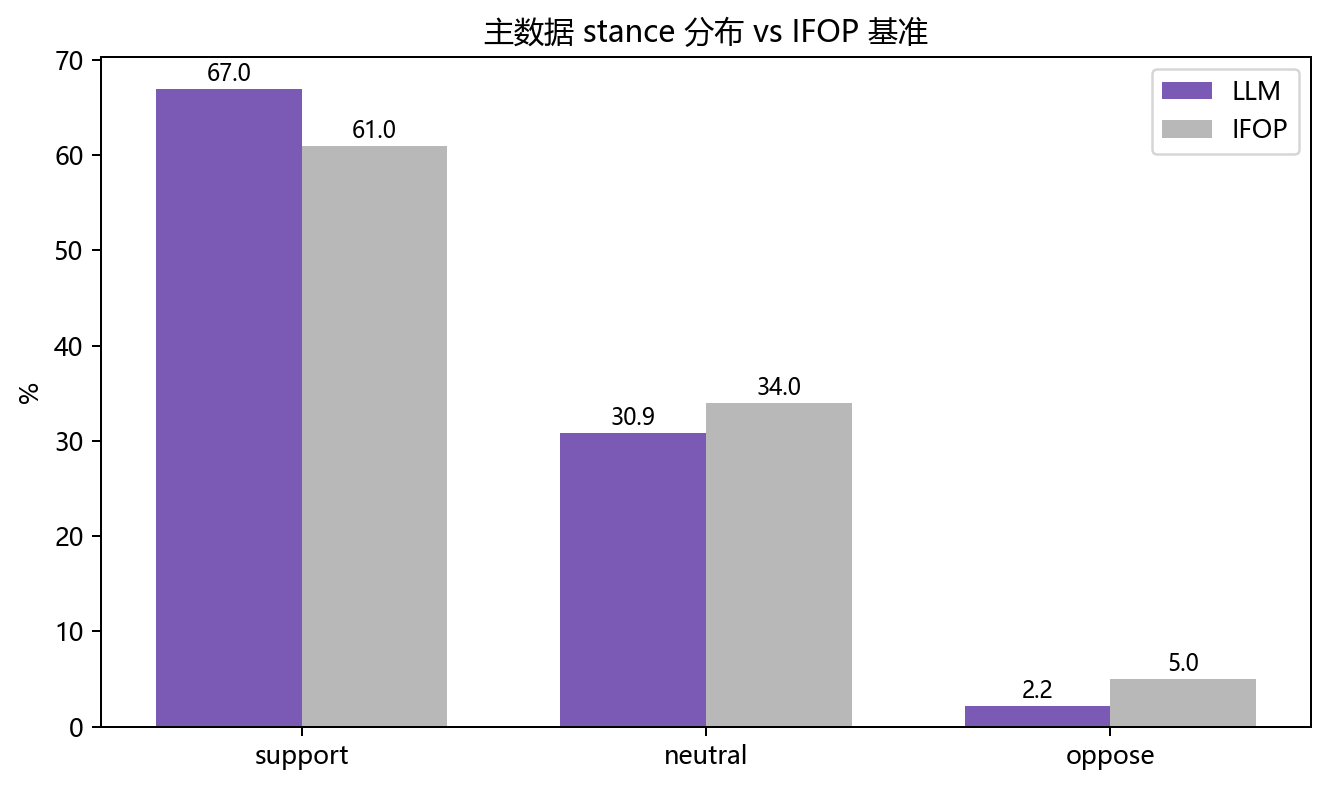
\includegraphics[width=\linewidth]{figures/stance_vs_ifop.png}
    \caption{Simulated stance vs. IFOP benchmark.}
  \end{subfigure}
  \hfill
  \begin{subfigure}{0.32\textwidth}
    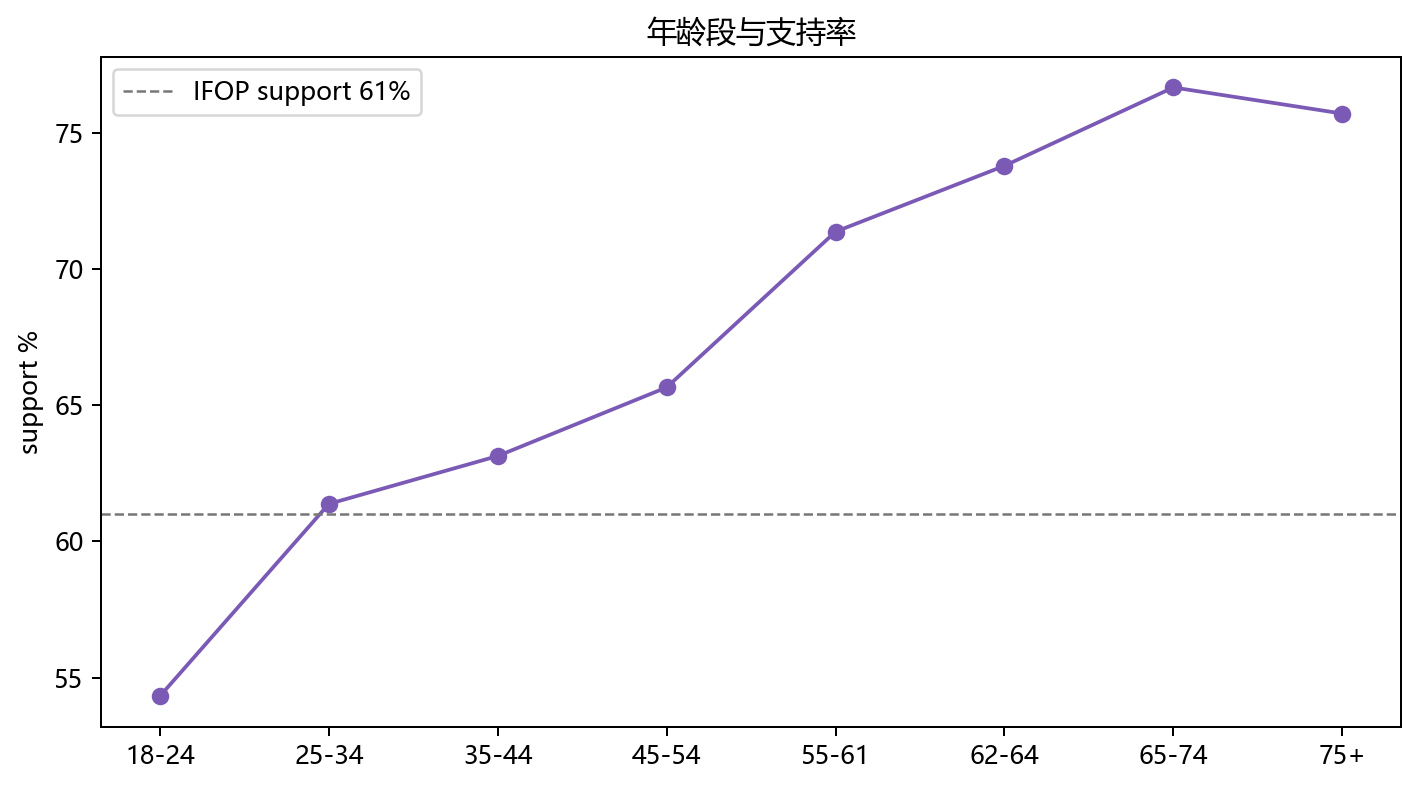
\includegraphics[width=\linewidth]{figures/age_group_support.png}
    \caption{Support rate by age group.}
  \end{subfigure}
  \hfill
  \begin{subfigure}{0.32\textwidth}
    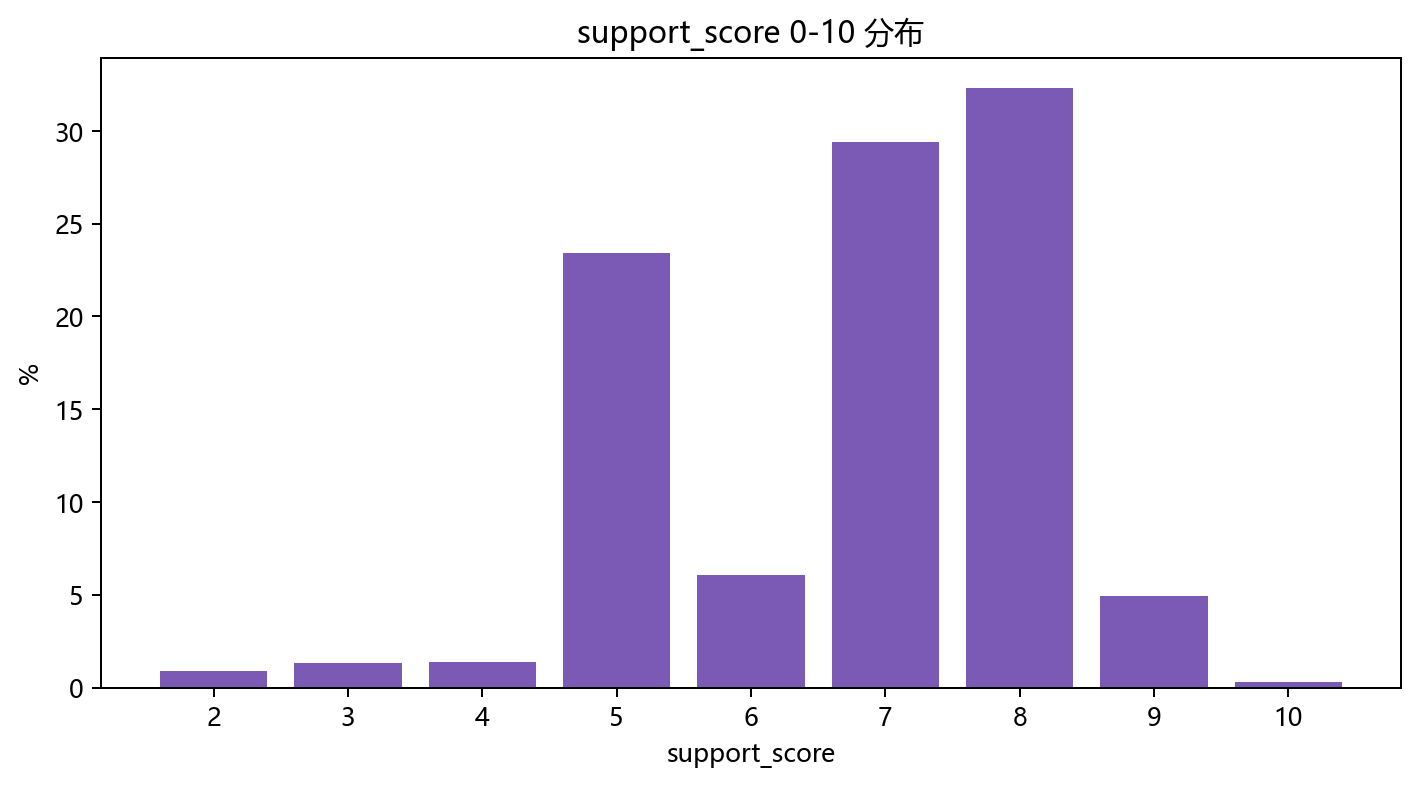
\includegraphics[width=\linewidth]{figures/score_distribution.png}
    \caption{Support-score distribution.}
  \end{subfigure}
  \caption{Exploratory analysis of the main simulated survey dataset. The aggregate pattern contains interpretable social signals, especially age-related support, but the score distribution is concentrated.}
  \label{fig:eda}
\end{figure*}

The exploratory findings justify predictive modeling but also foreshadow its limits. If age, occupation, and text fields contain meaningful signal, supervised models should recover some variation. If labels are noisy or key political variables are missing, model performance should plateau even when feature dimensionality increases.

\section{Feature Engineering and Modeling}
\subsection{First-Round Structured Features}
We first fixed the label $y$ and varied only the model input $X$. Four structured feature schemes were designed from simple to richer representations:

\begin{itemize}[leftmargin=*]
  \item \textbf{A0 Label}: low-complexity baseline using label/ordinal encodings.
  \item \textbf{A1 One-hot}: expands categorical variables to remove artificial ordering.
  \item \textbf{A2 Age+}: adds age mechanisms related to pension reform, such as age bins and near-retirement indicators.
  \item \textbf{A3 Social}: merges social categories such as occupation and education groups to reduce categorical noise.
\end{itemize}

Each feature scheme was evaluated with five model families: Linear Regression, Ridge Regression, Random Forest, XGBoost, and LightGBM. This yielded 20 structured-feature/model combinations under the same train-test split and evaluation metrics.

\begin{figure*}[t]
  \centering
  \begin{subfigure}{0.49\textwidth}
    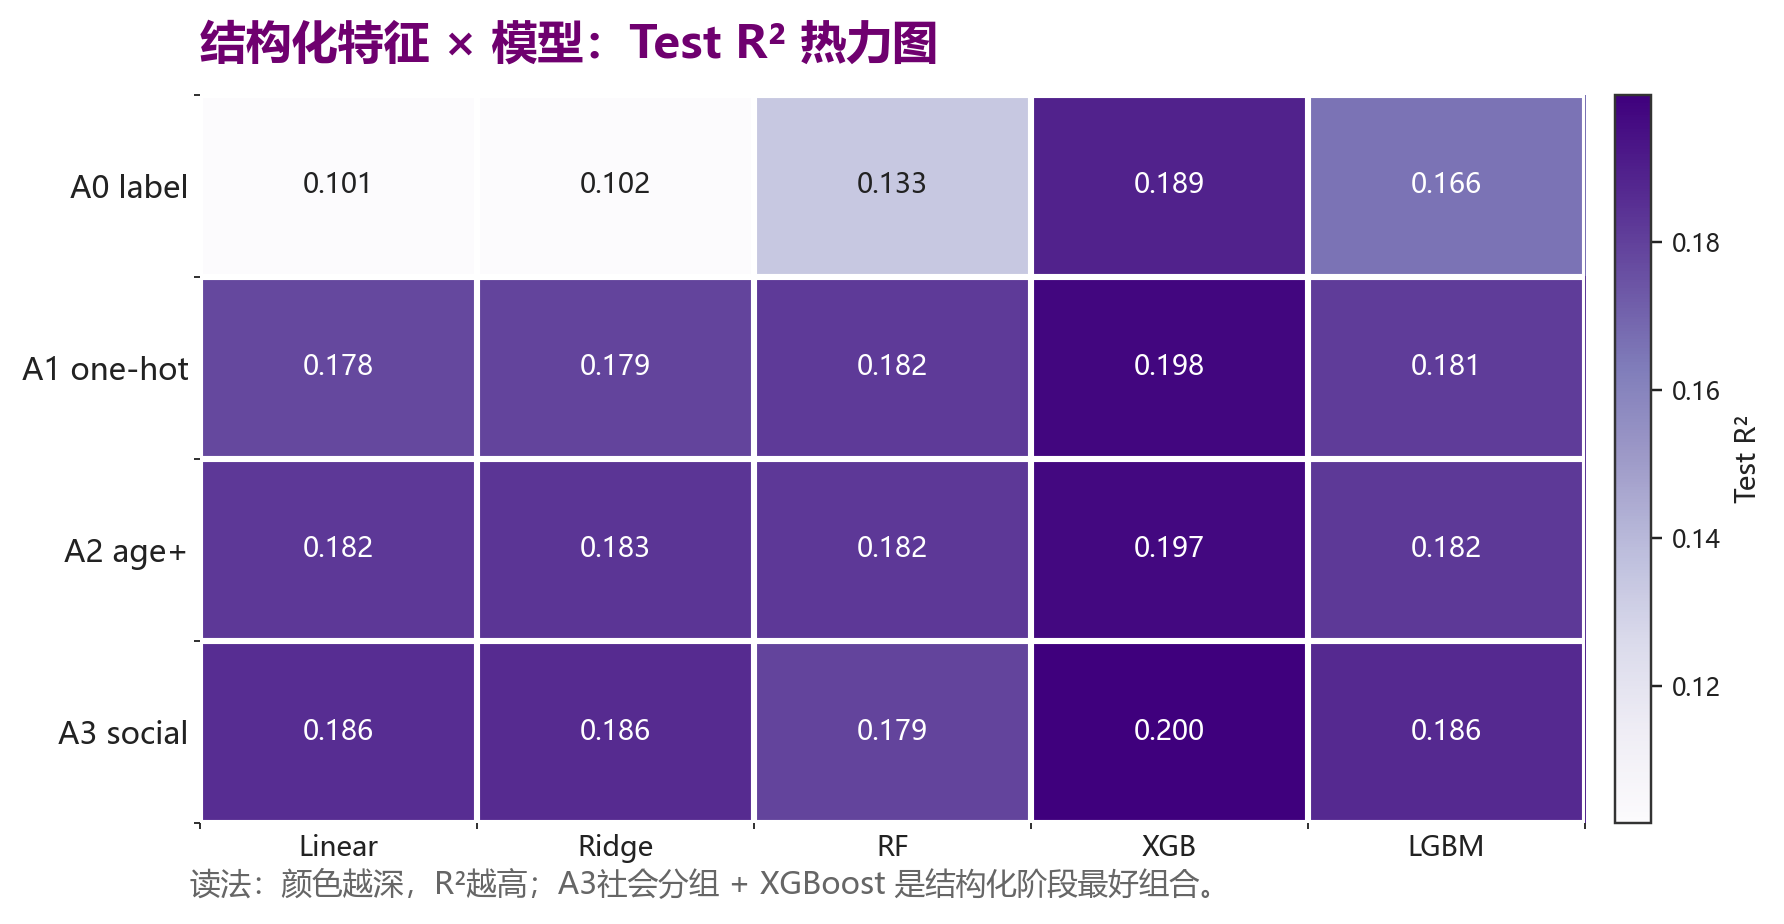
\includegraphics[width=\linewidth]{figures/structured_r2_heatmap.png}
    \caption{Structured features $\times$ regression models.}
  \end{subfigure}
  \hfill
  \begin{subfigure}{0.49\textwidth}
    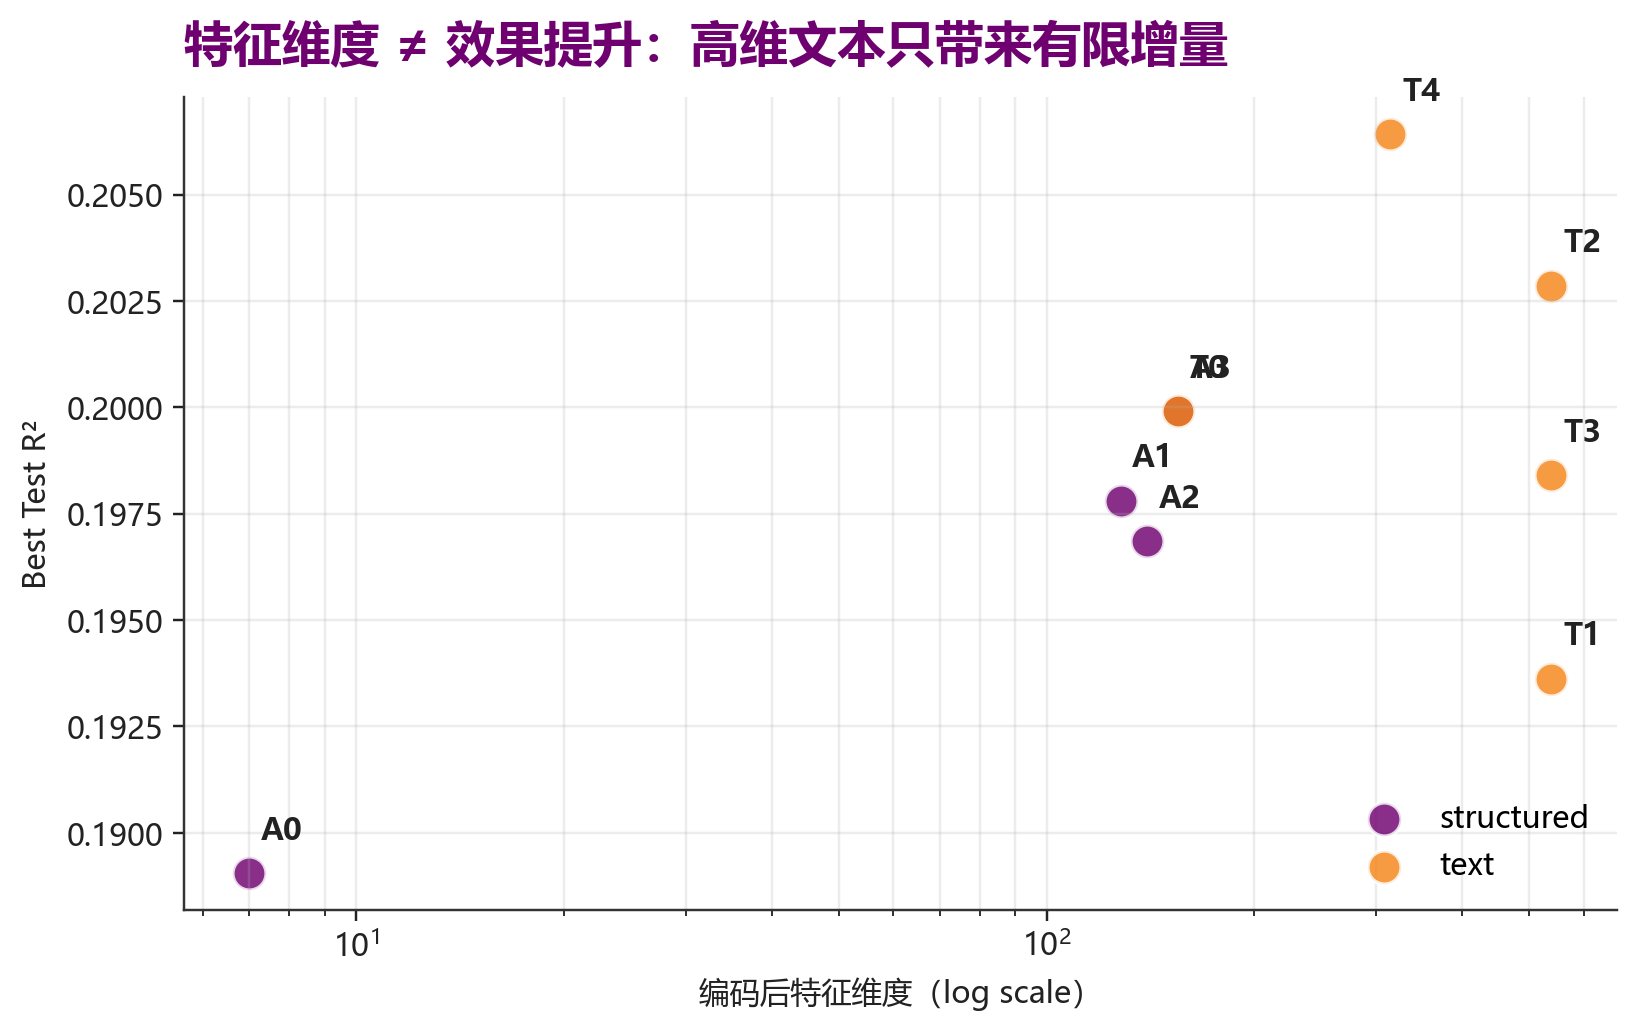
\includegraphics[width=\linewidth]{figures/feature_dimension_vs_r2.png}
    \caption{Feature dimensionality vs. best test $R^2$.}
  \end{subfigure}
  \caption{Modeling results show that richer features and more complex models improve performance initially, but quickly reach a plateau. The best structured-feature model is around $R^2=0.200$.}
  \label{fig:modeling1}
\end{figure*}

Figure~\ref{fig:modeling1} shows that the main improvement occurs when moving from simple linear/label baselines to boosted tree models. However, A1, A2, and A3 are close to one another, and the best structured result remains around $R^2=0.200$. This suggests that simply adding more structured categories or switching model families cannot fully explain individual-level variation in simulated support scores.

\subsection{Second-Round Text Features}
Because structured features plateaued, we next tested whether persona text fields provide additional information. We used A3 as the structured baseline and constructed five text-related schemes: T0 structured baseline, T1 full persona text embedding, T2 career text embedding, T3 lifestyle text embedding, and T4 field-level embeddings compressed with PCA. The PCA step reduces high-dimensional embedding redundancy while preserving broad semantic variation.

\begin{figure}[t]
  \centering
  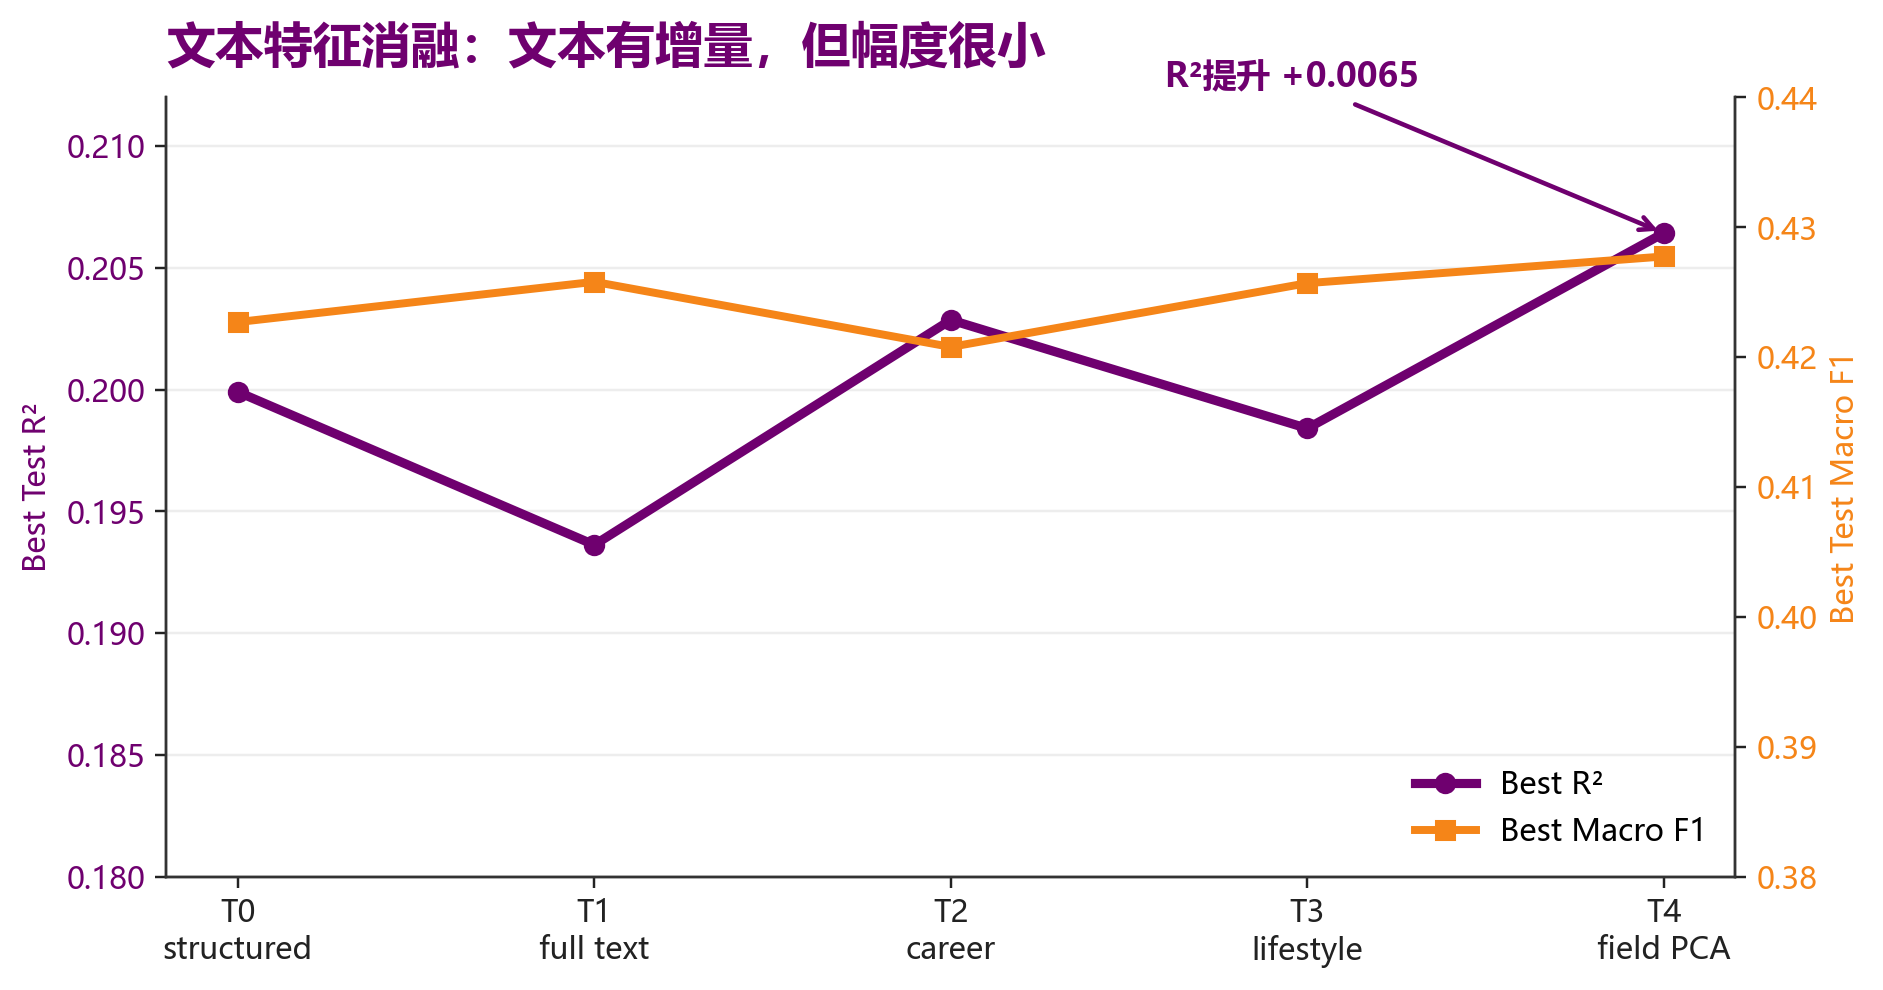
\includegraphics[width=\linewidth]{figures/text_feature_increment_lines.png}
  \caption{Text feature ablation. T4 field-level embeddings plus PCA produce the best result, but the improvement is small: test $R^2$ rises from about 0.200 to about 0.206.}
  \label{fig:textincrement}
\end{figure}

Figure~\ref{fig:textincrement} shows that textual features provide only limited incremental value. The best configuration, T4 with XGBoost, reaches approximately $R^2=0.206$. This small gain suggests that the persona text contains some useful semantic information, but lacks direct variables closer to attitude formation, such as ideology, union membership, pension dependency, party preference, or trust in government.

\section{Classification and Minority-Class Diagnosis}
Regression performance is only one part of the story. For the three-class stance label, overall accuracy can be misleading because support is the majority class. We therefore examine macro F1 and class-level F1.

\begin{figure}[t]
  \centering
  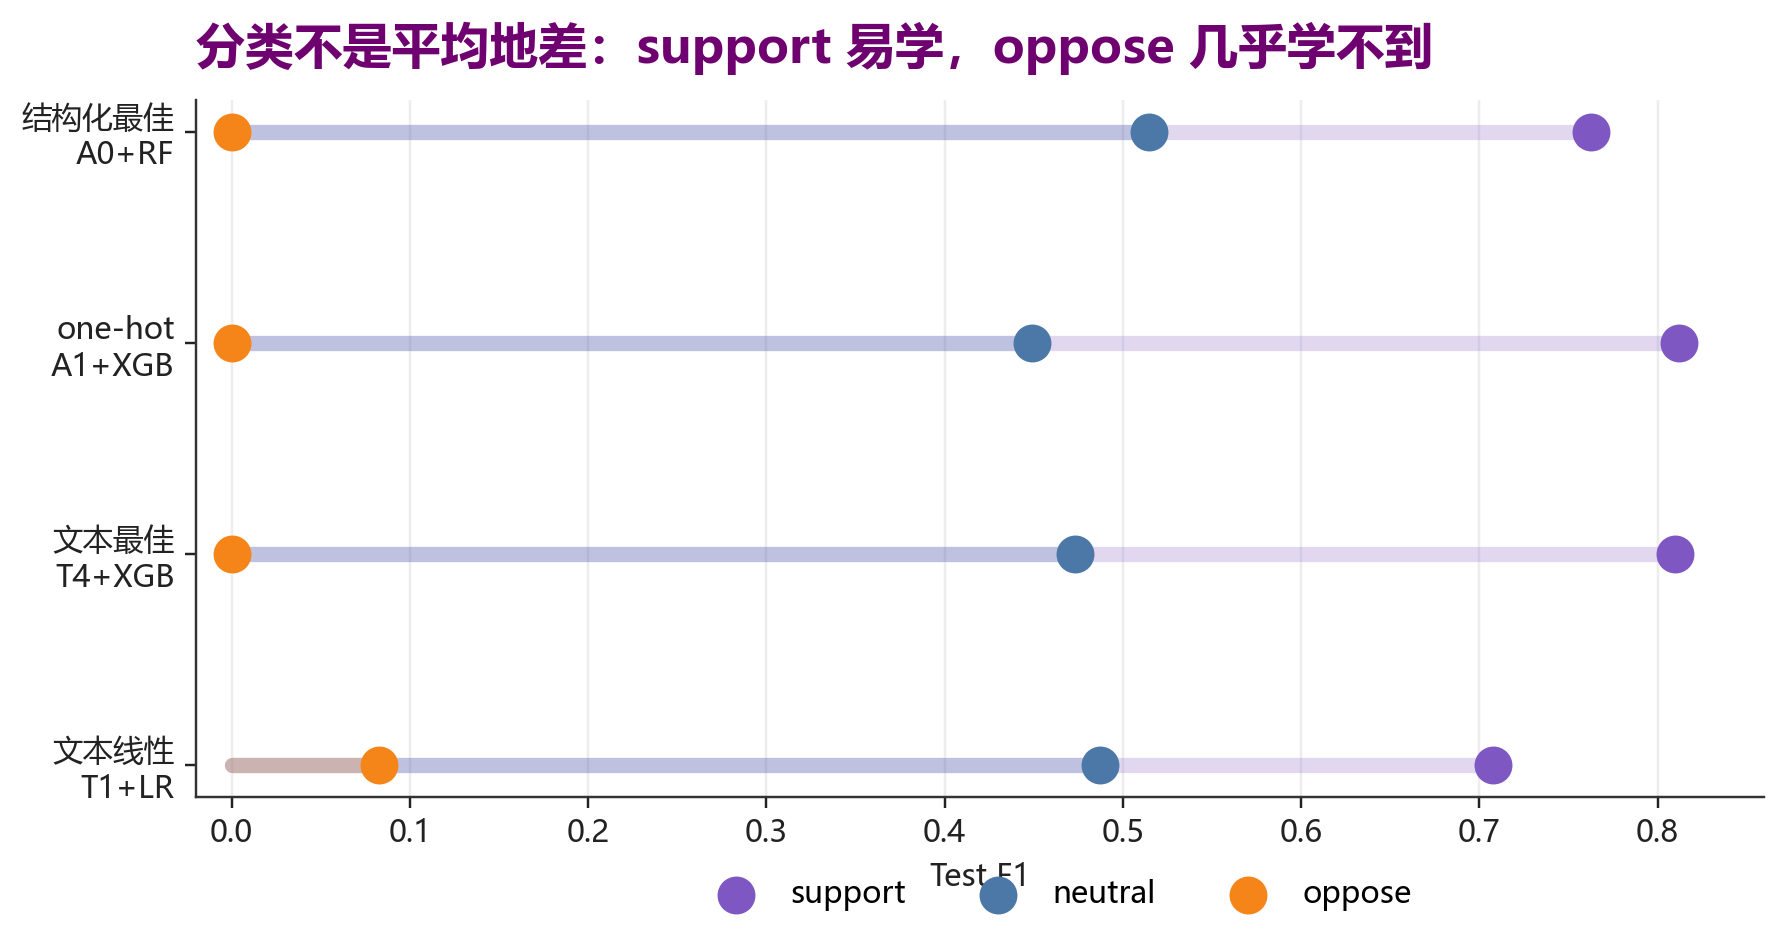
\includegraphics[width=\linewidth]{figures/class_f1_lollipop_selected_models.png}
  \caption{Class-level F1 for representative models. Support is consistently easier to learn; neutral is moderate; oppose is nearly unlearnable for most direct multiclass classifiers.}
  \label{fig:classf1}
\end{figure}

Figure~\ref{fig:classf1} reveals a sharp class imbalance in learnability. Support reaches relatively high F1, neutral remains moderate, and oppose is often near zero. The issue is therefore not merely that all predictions are poor; rather, the model learns the majority pattern but fails to form a stable boundary for the minority stance.

\subsection{Error Structure}
The confusion matrix in Figure~\ref{fig:diagnosis} shows the direct multiclass model's failure to predict oppose. True oppose cases are usually absorbed into neutral or support. Residual analysis further shows that errors are largest among oppose-labeled samples.

\begin{figure*}[t]
  \centering
  \begin{subfigure}{0.32\textwidth}
    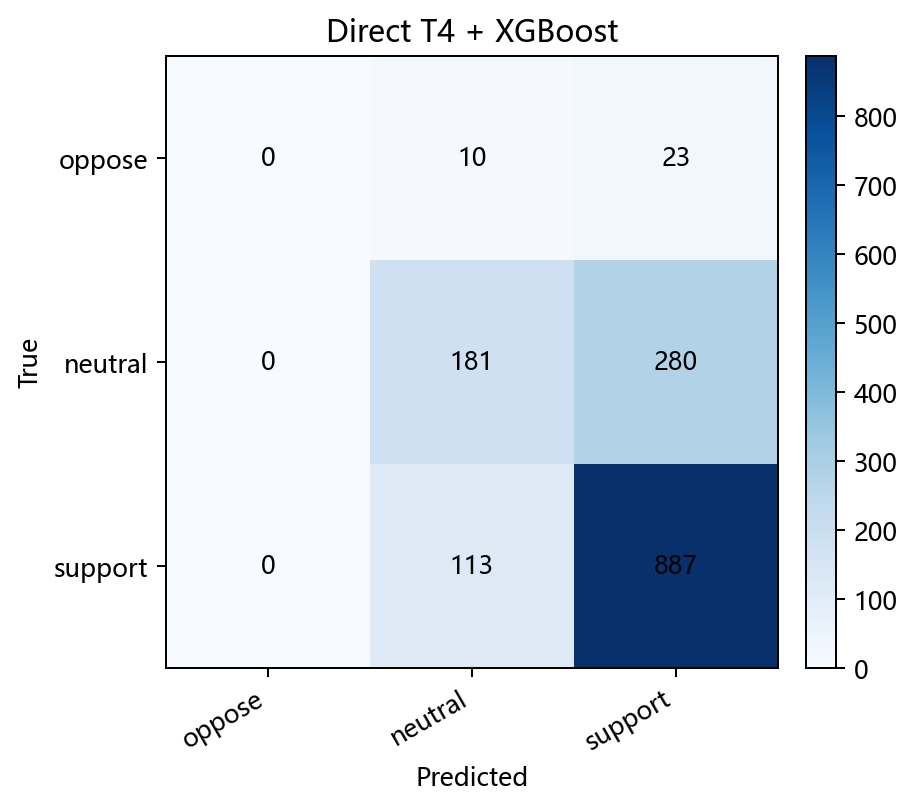
\includegraphics[width=\linewidth]{figures/direct_multiclass_confusion_matrix.png}
    \caption{Direct multiclass confusion matrix.}
  \end{subfigure}
  \hfill
  \begin{subfigure}{0.32\textwidth}
    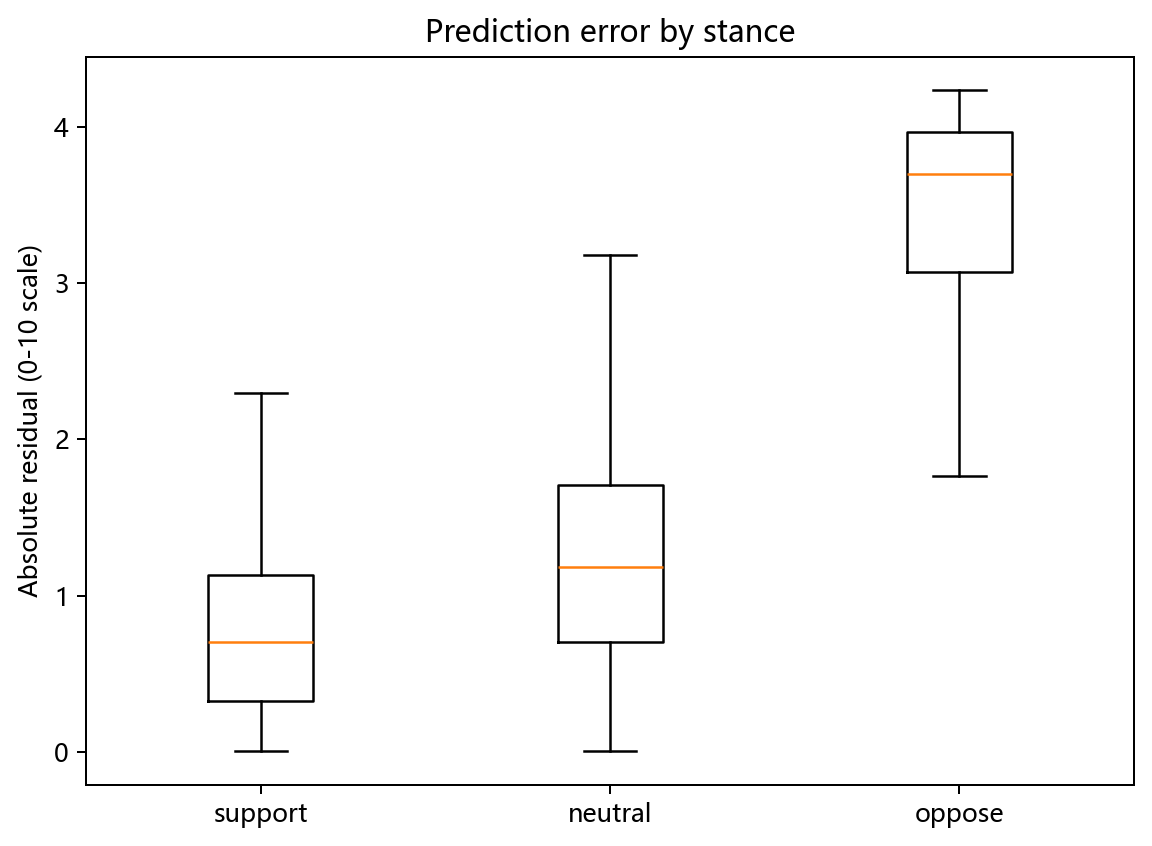
\includegraphics[width=\linewidth]{figures/absolute_residual_by_stance.png}
    \caption{Regression error by stance.}
  \end{subfigure}
  \hfill
  \begin{subfigure}{0.32\textwidth}
    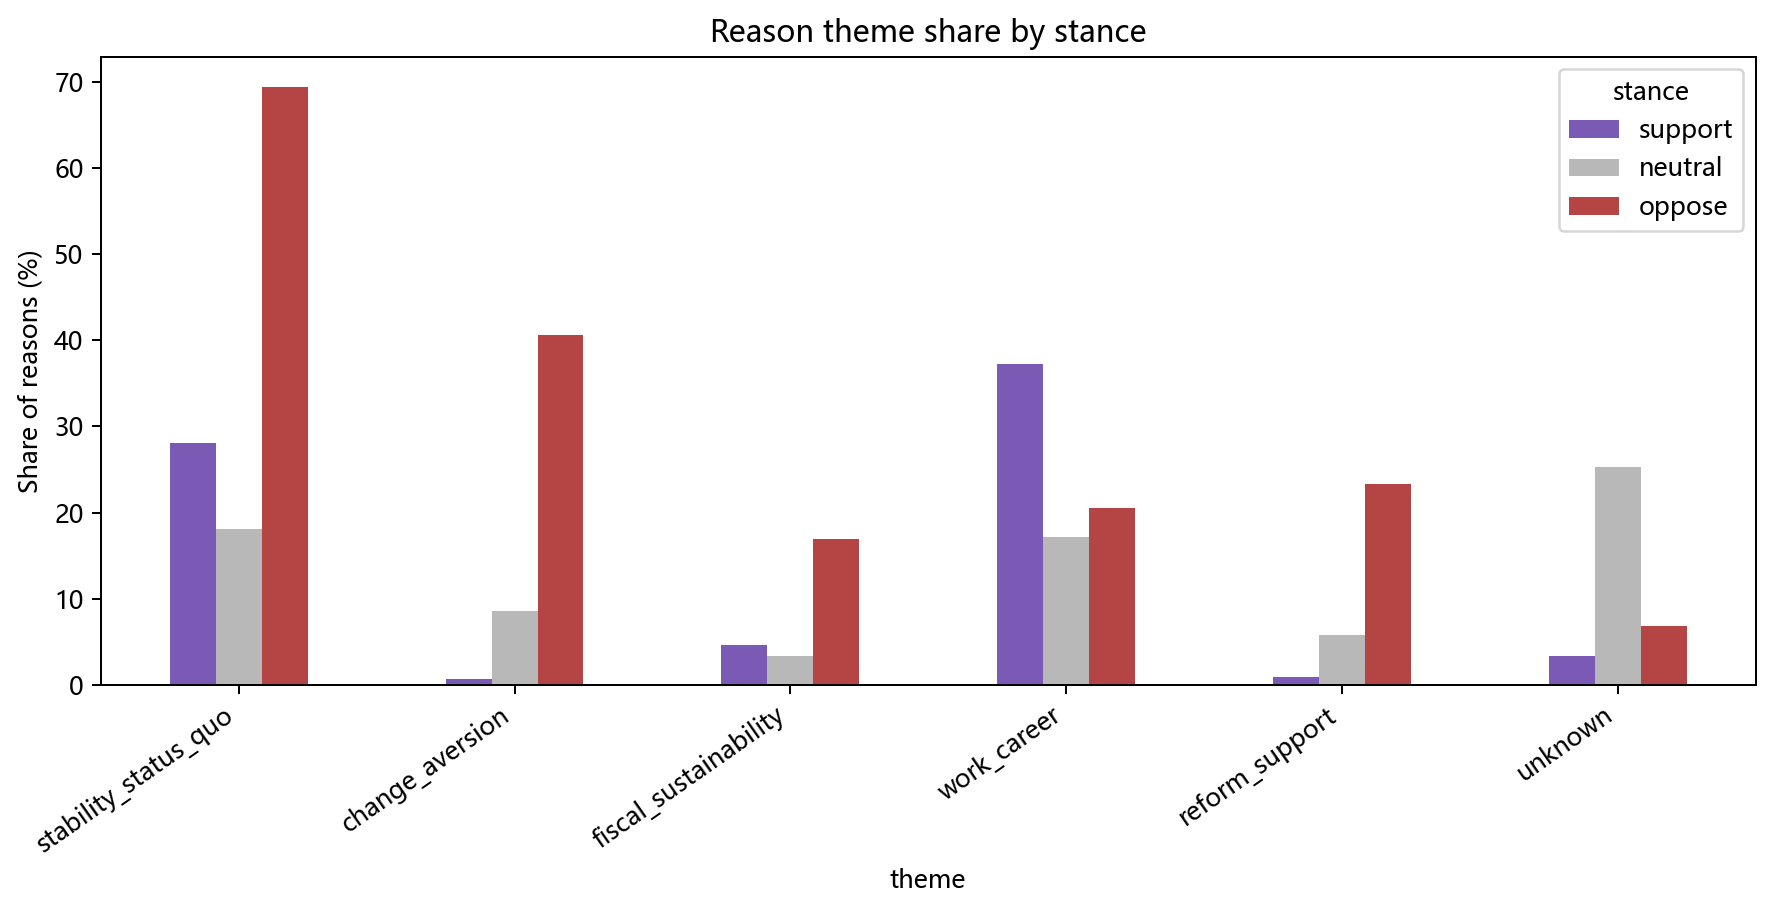
\includegraphics[width=\linewidth]{figures/reason_theme_by_stance.png}
    \caption{Reason-theme shares by stance.}
  \end{subfigure}
  \caption{Diagnostics for minority-class failure. Oppose is not only rare; its semantic boundary overlaps with neutral and support reasons, making it difficult for supervised models to recover.}
  \label{fig:diagnosis}
\end{figure*}

The reason-theme analysis suggests why. Oppose reasons are often concentrated around status quo preference and change aversion, but they also overlap with work, fiscal, reform, and age-related themes that appear in other stances. In other words, oppose is not a simple semantic opposite of support. It is a small, heterogeneous class with overlapping textual justifications.

\subsection{Label Stability Retest}
To test whether the problem lies only in sample size or also in label stability, we repeated LLM labeling for 300 personas, balanced across original stance categories, with two repeated calls per persona. The results show a clear stability gap: support labels reproduce well, while neutral and oppose are much less stable.

\begin{table}[t]
\centering
\caption{Label stability by original stance.}
\label{tab:stability}
\begin{tabular}{lrr}
\toprule
Original stance & Stance agreement & Score MAE (0--10) \\
\midrule
Support & 90.4\% & 0.71 \\
Neutral & 43.6\% & 1.54 \\
Oppose & 43.3\% & 2.02 \\
\bottomrule
\end{tabular}
\end{table}

Table~\ref{tab:stability} indicates that the downstream model is not trying to predict a perfectly stable label. If the LLM itself does not consistently reproduce neutral and oppose labels for the same persona, supervised models trained on those labels face an intrinsic ceiling.

\section{Optimization Attempts}
We tested several strategies to improve oppose recognition: probability thresholds, regression-threshold conversion, class weighting, and two-stage classification. These methods trade overall accuracy for minority-class recall.

\begin{figure}[t]
  \centering
  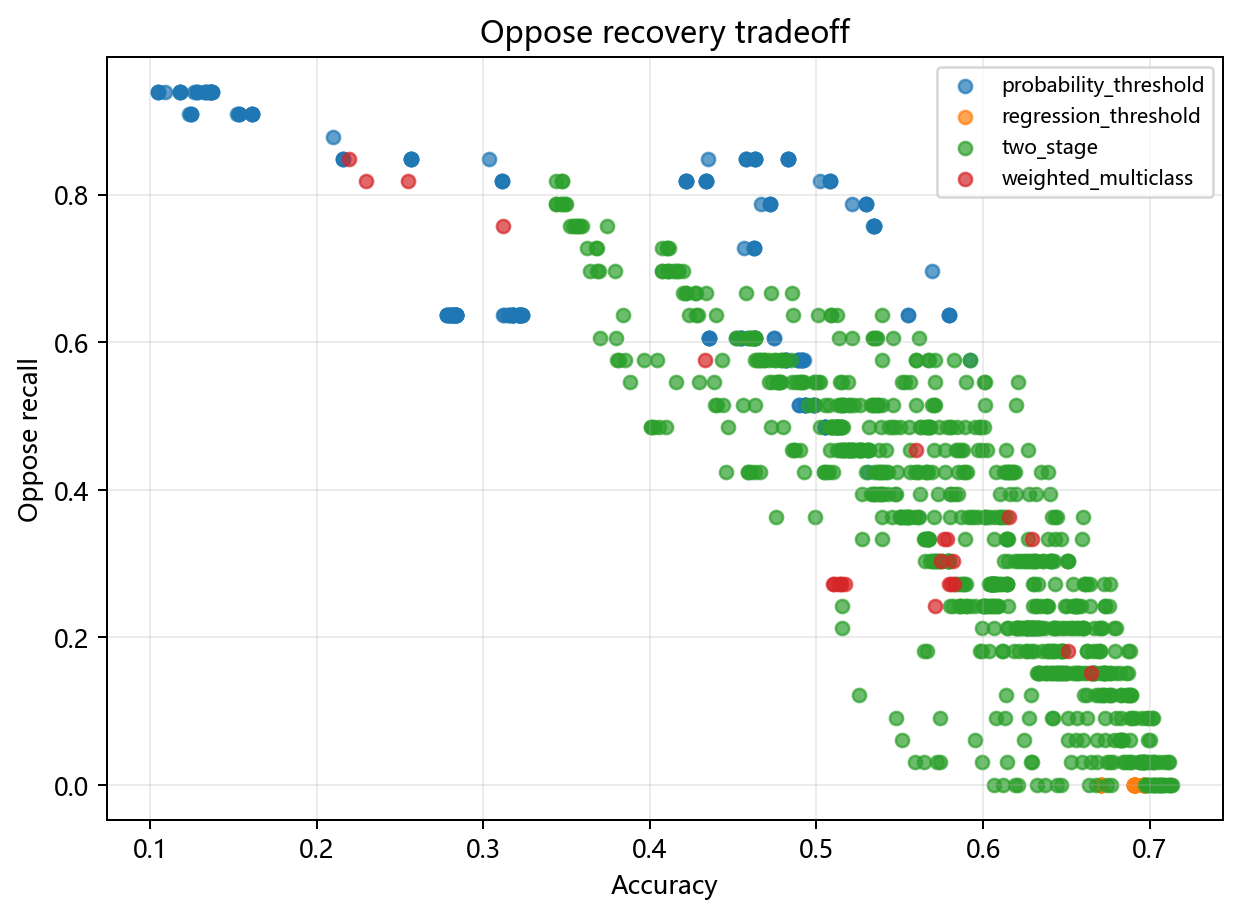
\includegraphics[width=\linewidth]{figures/oppose_recall_accuracy_tradeoff.png}
  \caption{Oppose recovery trade-off. Higher oppose recall generally requires sacrificing overall accuracy, indicating no free optimization point in the current data.}
  \label{fig:tradeoff}
\end{figure}

\begin{table}[t]
\centering
\caption{Representative optimization results on the test set.}
\label{tab:optimization}
\begin{tabular}{lrrrr}
\toprule
Method & Accuracy & Macro F1 & Oppose recall & Oppose F1 \\
\midrule
Original multiclass & 71.5\% & 42.8\% & 0.0\% & 0.0\% \\
Probability threshold & 59.2\% & 44.3\% & 57.6\% & 12.6\% \\
Class weighting & 66.5\% & 47.9\% & 15.2\% & 14.9\% \\
Two-stage classifier & 67.3\% & 48.7\% & 15.2\% & 16.9\% \\
\bottomrule
\end{tabular}
\end{table}

The two-stage classifier produces the best balanced improvement among the tested approaches, raising macro F1 and oppose F1 while maintaining moderate accuracy. However, the optimization results support the broader diagnosis: algorithmic adjustments can partially recover minority labels, but they cannot fully overcome missing features, overlapping reasons, class imbalance, and unstable LLM-generated labels.

\section{Discussion}
The project yields three substantive lessons.

First, persona-based LLM survey simulation is plausible at the aggregate level but fragile at the individual level. The simulated data roughly preserves the broad support/neutral/oppose ordering and produces interpretable age-related trends. Yet individual-level prediction remains limited, with the best regression model explaining only about one fifth of score variance.

Second, feature dimensionality is not the same as effective information. Text embeddings increase feature dimension substantially, but improve $R^2$ only from about 0.200 to 0.206. This suggests that the persona descriptions contain many socially rich details, but not necessarily the near-proximal political variables needed to explain pension-reform attitudes.

Third, minority-class failure is both a modeling issue and a data-generation issue. Oppose is rare, semantically heterogeneous, and less stable under repeated LLM calls. This aligns with broader concerns that synthetic respondents can flatten or misrepresent social groups \cite{wang2024replace,cheng2023marked}. Our results therefore support a cautious interpretation: the LLM-generated dataset should be analyzed as a simulated behavioral artifact, not as a substitute for real human survey evidence.

\section{Limitations}
Several limitations remain. The project uses one policy issue and one main LLM configuration, so generalization across topics, countries, and models is unknown. The IFOP benchmark provides an external aggregate reference, but it is not an individual-level ground truth. The persona dataset is synthetic and may already contain biases from its generation process. Finally, repeated-label experiments were limited in scale and should be expanded to better estimate reliability ceilings.

\section{Conclusion and Future Work}
This project constructed and analyzed a persona-based LLM public-opinion simulation pipeline for French pension reform. The main contribution is not a high-performing prediction model, but a diagnostic workflow for studying when LLM-generated respondents appear socially structured and when they break down. Future work should compare multiple LLMs, test multilingual prompts, expand to additional policy issues, add explicit political-attitude variables, increase test-retest reliability analysis, and explore multi-agent deliberation settings. The next stage should make simulated survey data closer to real public-opinion research while keeping its uncertainty visible.

\section*{Reproducibility Note}
The accompanying submission should include the frozen main dataset, analysis scripts, and all generated figures. The report itself does not require re-calling the LLM API. All downstream analyses should be reproducible from the saved dataset and fixed random seeds.

\bibliographystyle{plain}
\bibliography{references}

\end{document}

